\section{Produktfunktionen}
	% \input{3-Produktfunktionen}

		\subsection{Use Cases}
		% \input{3-1-Use_Cases}
		
		Die Abbildungen \ref{fig:3-1-robot-use-cases} und \ref{fig:3-1-server-use-cases} zeigen die Funktionalitäten der beiden Teilsysteme \emph{Robot} und \emph{Server}.
		
			\begin{figure}[H]
				\centering
				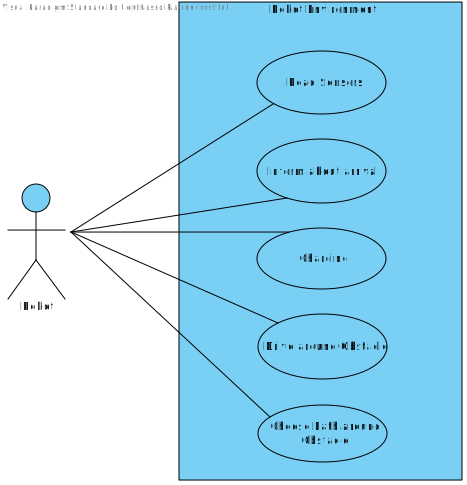
\includegraphics[width=0.8\textwidth]{img/1-Analyse-3-Robot}
				\caption{Use Case Diagramm 1: Use Cases des Roboters}
				\label{fig:3-1-robot-use-cases}
			\end{figure}

			\begin{figure}[H]
				\centering
				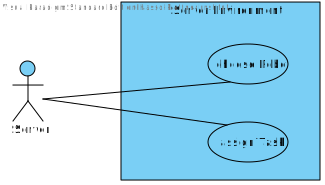
\includegraphics[width=0.8\textwidth]{img/1-Analyse-3-Server}
				\caption{Use Case Diagramm 2: Use Cases des Servers}
				\label{fig:3-1-server-use-cases}
			\end{figure}

			\begin{figure}[H]
				\centering
				\includegraphics[width=0.8\textwidth]{img/1-Analyse-3-Hospital}
				\caption{Use Case Diagramm 2: Use Cases des Hospitals}
				\label{fig:3-1-hospital-use-cases}
			\end{figure}

		\pagebreak

		\subsection{Beschreibung zu Use Case \emph{1}: Drive to Destination}

			\subsubsection*{Charakterisierende Informationen}

			\begin{table}[H]
				\centering
				\begin{tabularx}{\textwidth}{@{}p{5cm}X@{}}
				\toprule
				\textbf{Übergeordneter elementarer Geschäftsprozess:} & Drive to Destination\\ \midrule
				\textbf{Ziel des Use Cases:} & \emph{Robot} fährt eine \emph{Destination} an\\ \midrule
				\textbf{Umgebende Systemgrenze:} & \emph{Robot} \\ \midrule
				\textbf{Vorbedingung:} & Ein spezieller \emph{Robot} wurde vom Server ausgewählt und sein Akkustand ist hoch genug um den Auftrag auszuführen \\ \midrule
				\textbf{Nachbedingung bei erfolgreicher Ausführung:} & \emph{Robot} ist an der \emph{Destination} angekommen und meldet dies dem \emph{Server} \\ \midrule
				\textbf{Beteiligte Nutzer:} & \emph{Robot} \\ \midrule
				\textbf{Auslösendes Ereignis:} & \emph{Robot} hat eine \emph{Destination} erhalten. \\
				\bottomrule
				\end{tabularx}
			\end{table}

			Dieser Use Case wird dann benutzt, wenn ein \emph{Robot} eine aktuelle
			\emph{Destination} hat. In dieser Ausbaustufe betrachten wir lediglich das Anfahren
			einer \emph{Destination} von einem \emph{Robot}. Der \emph{Robot} dreht sich zunächst in die
			Richtung der \emph{Destination} und fährt so lange in Luftlinie, bis er entweder
			ankommt oder ein Hindernis erkennt. Ein konkreter Prozess zur Erkennung
			eines Hindernisses ist eine Entwurfsentscheidung und wird daher noch
			nicht berücksichtigt. Wenn der \emph{Robot} ein \emph{Obstacle} erkennt, dann
			sucht er einen guten Weg um das Hindernis herum. Wie er diesen Weg sucht
			ist auch zunächst eine Entwurfsentscheidung und noch nicht relevant. Auf
			diesem Weg umfährt er dann das \emph{Obstacle} und nimmt erneut die Fahrt auf
			Luftlinie auf.

			\subsubsection*{Szenario für den Standardablauf (Erfolg)}

			\begin{table}[H]
				\centering
				\begin{tabularx}{\textwidth}{@{}cp{2cm}X@{}}
				\toprule
				Schritt & Nutzer & Beschreibung der Aktivität \\ \midrule
				1 & Robot & \emph{Robot} dreht sich in Richtung aktueller \emph{Destination} \\
				2 & Robot & \emph{Robot} fährt geradeaus \\
				3 & Robot & \emph{Robot} erreicht \emph{Destination} \\
				\bottomrule
				\end{tabularx}
			\end{table}

			\subsubsection*{Szenarien für alternative Abläufe\\ (Misserfolg oder Umwege zum Erfolg)}

			\begin{table}[H]
				\centering
				\begin{tabularx}{\textwidth}{@{}cp{6cm}X@{}}
				\toprule
				Schritt & Bedingung für Alternative & Beschreibung der Aktivität \\ \midrule
				3 & \emph{Robot} erkennt ein \emph{Obstacle} zwischen auf seinem Weg zum Ziel & \emph{Robot} sucht sich einen Umweg um das \emph{Obstacle}, umfährt das \emph{Obstacle} und nimmt schließlich Standardablauf wieder auf \\
				\bottomrule
				\end{tabularx}
			\end{table}

			%\subsubsection*{Beschreibung des allgemeinen Ablaufes}
			
		\pagebreak

		\subsection{Beschreibung zu Use Case \emph{2}: Read Sensors}

			\subsubsection*{Charakterisierende Informationen}

			\begin{table}[H]
				\centering
				\begin{tabularx}{\textwidth}{@{}p{5cm}X@{}}
				\toprule
				\textbf{Übergeordneter elementarer Geschäftsprozess:} & Choose Robot\\ \midrule
				\textbf{Ziel des Use Cases:} & \emph{Robot} kann über seinen Akkustand und seine Position Auskunft geben\\ \midrule
				\textbf{Umgebende Systemgrenze:} & \emph{Robot} \\ \midrule
				\textbf{Vorbedingung:} & \emph{Robot} hat eine Anfrage vom \emph{Server} erhalten \\ \midrule
				\textbf{Nachbedingung bei erfolgreicher Ausführung:} & \emph{Robot} schickt die ermittelten Informationen an den \emph{Server} \\ \midrule
				\textbf{Beteiligte Nutzer:} & \emph{Robot} \\ \midrule
				\textbf{Auslösendes Ereignis:} & \emph{Robot} hat eine Anfrage vom \emph{Server} erhalten, seine Sensoren zu lesen und sie dem \emph{Server} zu schicken \\
				\bottomrule
				\end{tabularx}
			\end{table}

			Im Rahmen vom Geschäftsprozess \emph{Choose Robot} sammelt der \emph{Server}
			Informationen über jeden \emph{Robot}. Diese Informationen (z.B
			Akkustand, aktuelle Position, ob der \emph{Robot} gerade ein Ziel verfolgt)
			kann der \emph{Robot} von seinen Hardware-Schnittstellen anfordern. Dieses
			Use Case wird dann ausgefüht, wenn der \emph{Robot} eine Anfrage vom
			Server erhält, seine Sensoren zu lesen, und endet damit, dass der \emph{Robot}
			die zusammengefassten Informationen an den \emph{Server} schickt.

			\subsubsection*{Szenario für den Standardablauf (Erfolg)}

			\begin{table}[H]
				\centering
				\begin{tabularx}{\textwidth}{@{}cp{2cm}X@{}}
				\toprule
				Schritt & Nutzer & Beschreibung der Aktivität \\ \midrule
				1 & Robot & \emph{Robot} erhält Anfrage vom \emph{Server} \\
				2 & Robot & \emph{Robot} sammelt Informationen von seiner Hardwareschnittstelle und fasst sie zusammen \\
				3 & Robot & \emph{Robot} schickt zusammengefasste Informationen an den Server \\
				\bottomrule
				\end{tabularx}
			\end{table}

			%\subsubsection*{Beschreibung des allgemeinen Ablaufes}
			
		\pagebreak

		\subsection{Beschreibung zu Use Case \emph{3}: Charging}

			\subsubsection*{Charakterisierende Informationen}

			\begin{table}[H]
				\centering
				\begin{tabularx}{\textwidth}{@{}p{5cm}X@{}}
				\toprule
				\textbf{Übergeordneter elementarer Geschäftsprozess:} & Drive to Destination\\ \midrule
				\textbf{Ziel des Use Cases:} & Ziel ist es, dem \emph{Robot} zu ermöglichen seine Ladestation anzufahren\\ \midrule
				\textbf{Umgebende Systemgrenze:} & \emph{Robot}\\ \midrule
				\textbf{Vorbedingung:} & Der \emph{Robot} erreicht sein vorgegebenes Ziel\\ \midrule
				\textbf{Nachbedingung bei erfolgreicher Ausführung:} & Der \emph{Robot} erreicht seine Ladestation\\ \midrule
				\textbf{Beteiligte Nutzer:} & \emph{Robot}\\ \midrule
				\textbf{Auslösendes Ereignis:} & \emph{Robot} erreicht \emph{Destination} (Use-Case)\\
				\bottomrule
				\end{tabularx}
			\end{table}

			Jedem Robot wird, laut Aufgabenstellung, eine feste Ladestation zugewiesen. Der Robot fährt vollständig autonom diese Ladestation an. Daher ist keine Kommunikation mit dem Server notwendig.

			\subsubsection*{Szenario für den Standardablauf (Erfolg)}

			\begin{table}[H]
				\centering
				\begin{tabularx}{\textwidth}{@{}cp{2cm}X@{}}
				\toprule
				Schritt & Nutzer & Beschreibung der Aktivität \\ \midrule
				1 & Robot & \emph{Robot} erreicht Ziel \\
				2 & Robot & \emph{Robot} fährt zur Ladestation \\
				3 & Robot & \emph{Robot} erreicht Ladestation und lädt sich auf \\
				4 & Robot & \emph{Robot} erhält neues Ziel und fährt dorthin \\
				\bottomrule
				\end{tabularx}
			\end{table}

			%\subsubsection*{Beschreibung des allgemeinen Ablaufes}
			
		\pagebreak

		\subsection{Beschreibung zu Use Case \emph{4}: Choose Robot}

			\subsubsection*{Charakterisierende Informationen}

			\begin{table}[H]
				\centering
				\begin{tabularx}{\textwidth}{@{}p{5cm}X@{}}
				\toprule
				\textbf{Übergeordneter elementarer Geschäftsprozess:} & Choose Robot \\ \midrule
				\textbf{Ziel des Use Cases:} & passenden \emph{Robot} für die durch den \emph{Server} gesendete \emph{Destination} auswählen\\ \midrule
				\textbf{Umgebende Systemgrenze:} & \emph{Robot} und \emph{Server} \\ \midrule
				\textbf{Vorbedingung:} & \emph{Server} hat eine neue \emph{Destination} bekommen\\ \midrule
				\textbf{Nachbedingung bei erfolgreicher Ausführung:} & dem ausgewählten \emph{Robot} wird die Task übertragen\\ \midrule
				\textbf{Beteiligte Nutzer:} & \emph{Robot} und \emph{Server}\\ \midrule
				\textbf{Auslösendes Ereignis:} & \emph{Server} empfängt neue \emph{Destination}\\
				\bottomrule
				\end{tabularx}
			\end{table}

			\subsubsection*{Szenario für den Standardablauf (Erfolg)}

			\begin{table}[H]
				\centering
				\begin{tabularx}{\textwidth}{@{}cp{2cm}X@{}}
				\toprule
				Schritt & Nutzer & Beschreibung der Aktivität \\ \midrule
				1 & Server & \emph{Server} sendet Anfragen an alle \emph{Robots} \\
				2 & Robot & \emph{Robots} empfangen Anfrage und führen dann den Use-Case „read Sensor“ aus \\
				3 & Robot & \emph{Robots} senden ihre ermittelten Sensorwerte an den \emph{Server}\\
				4 & Server & \emph{Server} empfängt Daten und wählt den am Besten geeigneten \emph{Robot} aus \\
				\bottomrule
				\end{tabularx}
			\end{table}

			%\subsubsection*{Beschreibung des allgemeinen Ablaufes}
			
		\pagebreak

		\subsection{Beschreibung zu Use Case \emph{5}: Assign Task}

			\subsubsection*{Charakterisierende Informationen}

			\begin{table}[H]
				\centering
				\begin{tabularx}{\textwidth}{@{}p{5cm}X@{}}
				\toprule
				\textbf{Übergeordneter elementarer Geschäftsprozess:} & Choose Robot  \\ \midrule
				\textbf{Ziel des Use Cases:} & \emph{Robot} den Task (die \emph{Destination}) zuweisen\\ \midrule
				\textbf{Umgebende Systemgrenze:} & \emph{Server} und \emph{Robot} \\ \midrule
				\textbf{Vorbedingung:} & „choose Robot“ hat am Besten geeigneten \emph{Robot} gefunden und ausgewählt\\ \midrule
				\textbf{Nachbedingung bei erfolgreicher Ausführung:} & ausgewähler \emph{Robot} steuert die \emph{Destination} an\\ \midrule
				\textbf{Beteiligte Nutzer:} & \emph{Server} und \emph{Robot}\\ \midrule
				\textbf{Auslösendes Ereignis:} & im Use-Case „choose Robot“ wurde passender \emph{Robot} ausgewählt\\
				\bottomrule
				\end{tabularx}
			\end{table}

			\subsubsection*{Szenario für den Standardablauf (Erfolg)}

			\begin{table}[H]
				\centering
				\begin{tabularx}{\textwidth}{@{}cp{2cm}X@{}}
				\toprule
				Schritt & Nutzer & Beschreibung der Aktivität \\ \midrule
				1 & Server & \emph{Server} überträgt ausgewähltem \emph{Robot} den Task \\
				\bottomrule
				\end{tabularx}
			\end{table}

			%\subsubsection*{Beschreibung des allgemeinen Ablaufes}

	\pagebreak


		\subsection{Beschreibung zu Use Case \emph{6}: Check Availability}

			\subsubsection*{Charakterisierende Informationen}

			\begin{table}[H]
				\centering
				\begin{tabularx}{\textwidth}{@{}p{5cm}X@{}}
				\toprule
				\textbf{Übergeordneter elementarer Geschäftsprozess:} & Take Patient to Hospital  \\ \midrule
				\textbf{Ziel des Use Cases:} & \emph{Hospital} erfährt, ob ein Auftrag vom System entgegengenommen werden kann. \midrule
				\textbf{Umgebende Systemgrenze:} &  \\ \midrule
				\textbf{Vorbedingung:} &  \midrule
				\textbf{Nachbedingung bei erfolgreicher Ausführung:} & Das System führt den Auftrag aus und bringt den \emph{Patient} in das \emph{Hospital} \\ \midrule
				\textbf{Beteiligte Nutzer:} & \emph{Hospital} und \emph{Server}\\ \midrule
				\textbf{Auslösendes Ereignis:} & \emph{Hospital} hat einen neuen Auftrag\\
				\bottomrule
				\end{tabularx}
			\end{table}

			Das \emph{Hospital} fragt laut Aufgabenstellung an dem zu modellierenden System an, ob ein \emph{Robot} verfügbar ist, um einen \emph{Patient} anzufahren und ins \emph{Hospital} zu bringen. Dazu wird vom \emph{Server} unter anderem der Use Case \emph{Choose Robot} ausgeführt. Es kann passieren, dass kein \emph{Robot} verfügbar ist, dann soll wie in der Aufgabenstellung beschrieben der Auftrag vom System abgelehnt werden. Was das \emph{Hospital} dann für Maßnahmen ergreift, wird hier nicht modelliert da es nicht teil des Systems ist.

			%\subsubsection*{Beschreibung des allgemeinen Ablaufes}

	\pagebreak
